\chapter{Meassurements}

\begin{figure}[H]
\centering
\begin{subfigure}[b]{0.48\textwidth}
                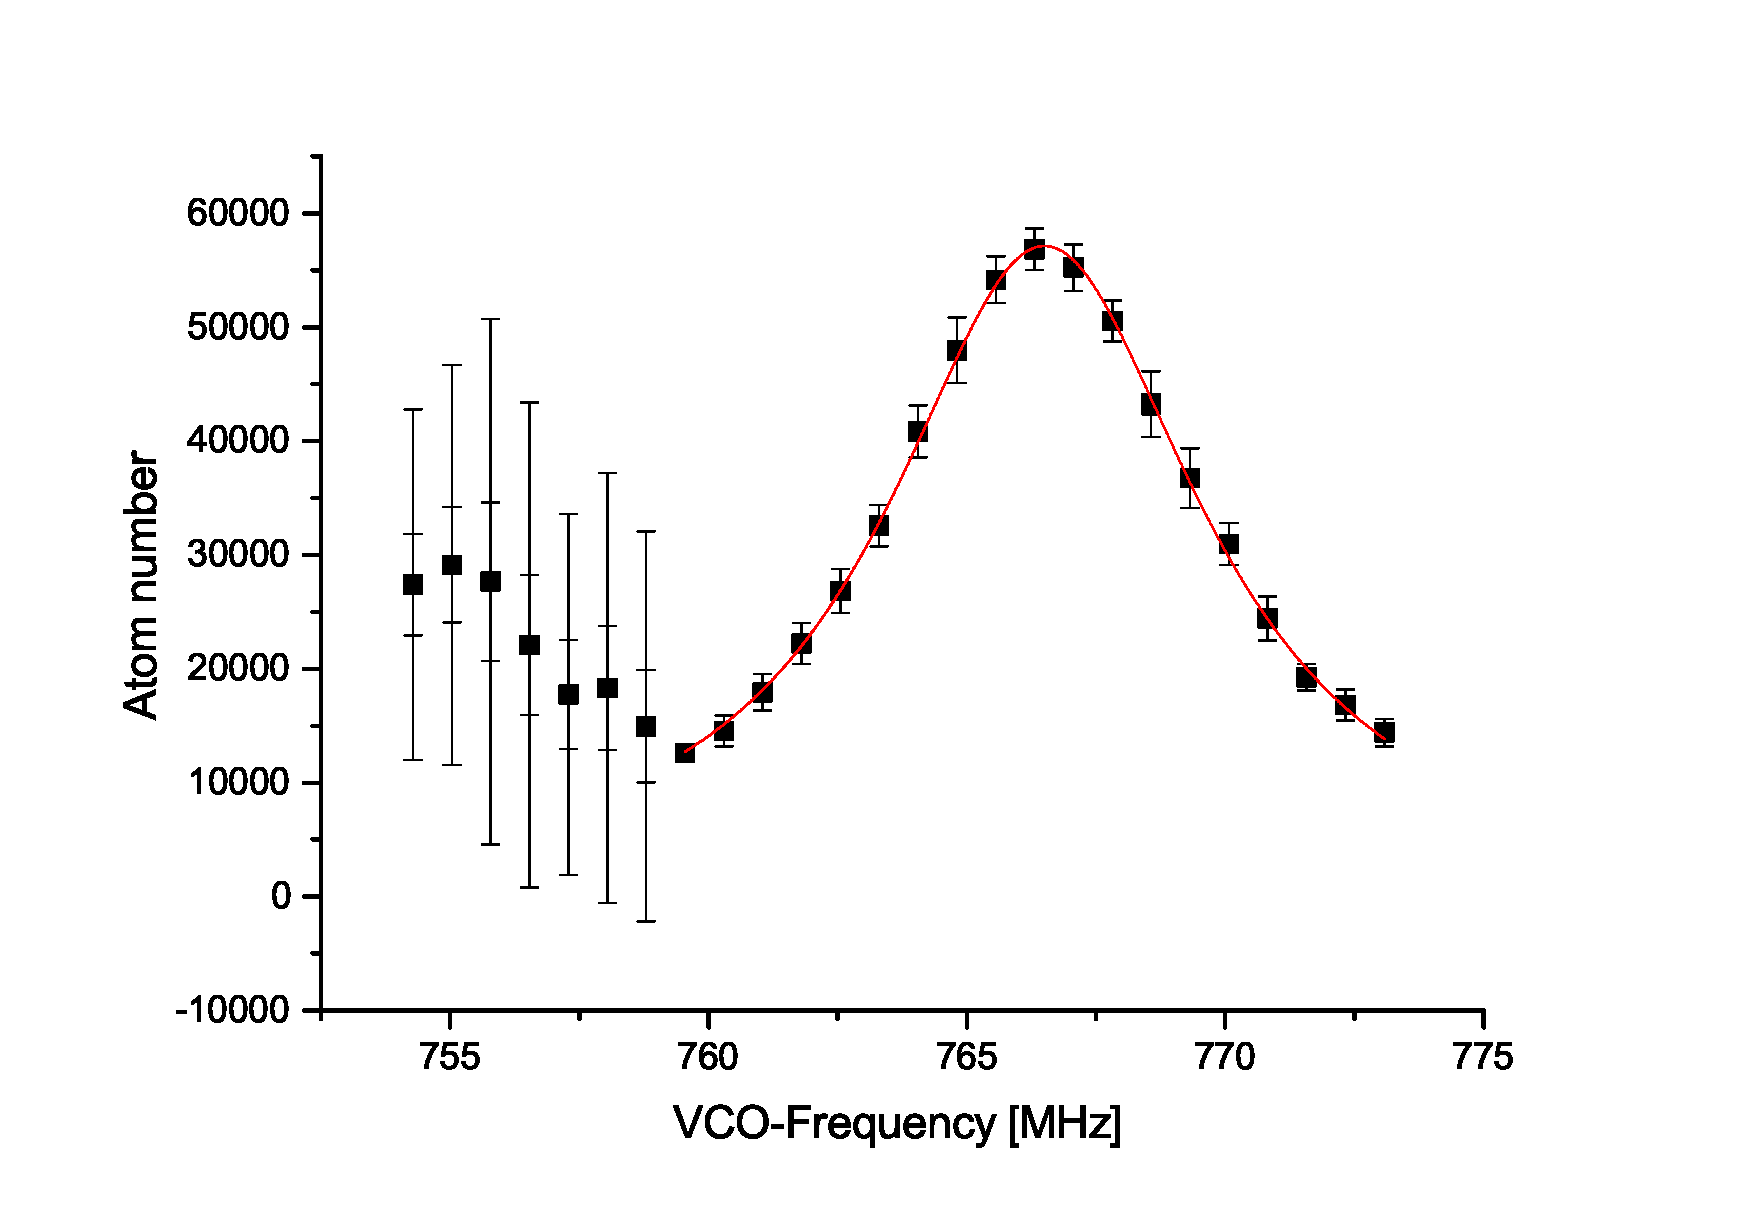
\includegraphics[width=\textwidth]{withoutodt}
                \caption{Dipole-trap turned off.}
\end{subfigure}
\begin{subfigure}[b]{0.48\textwidth}
               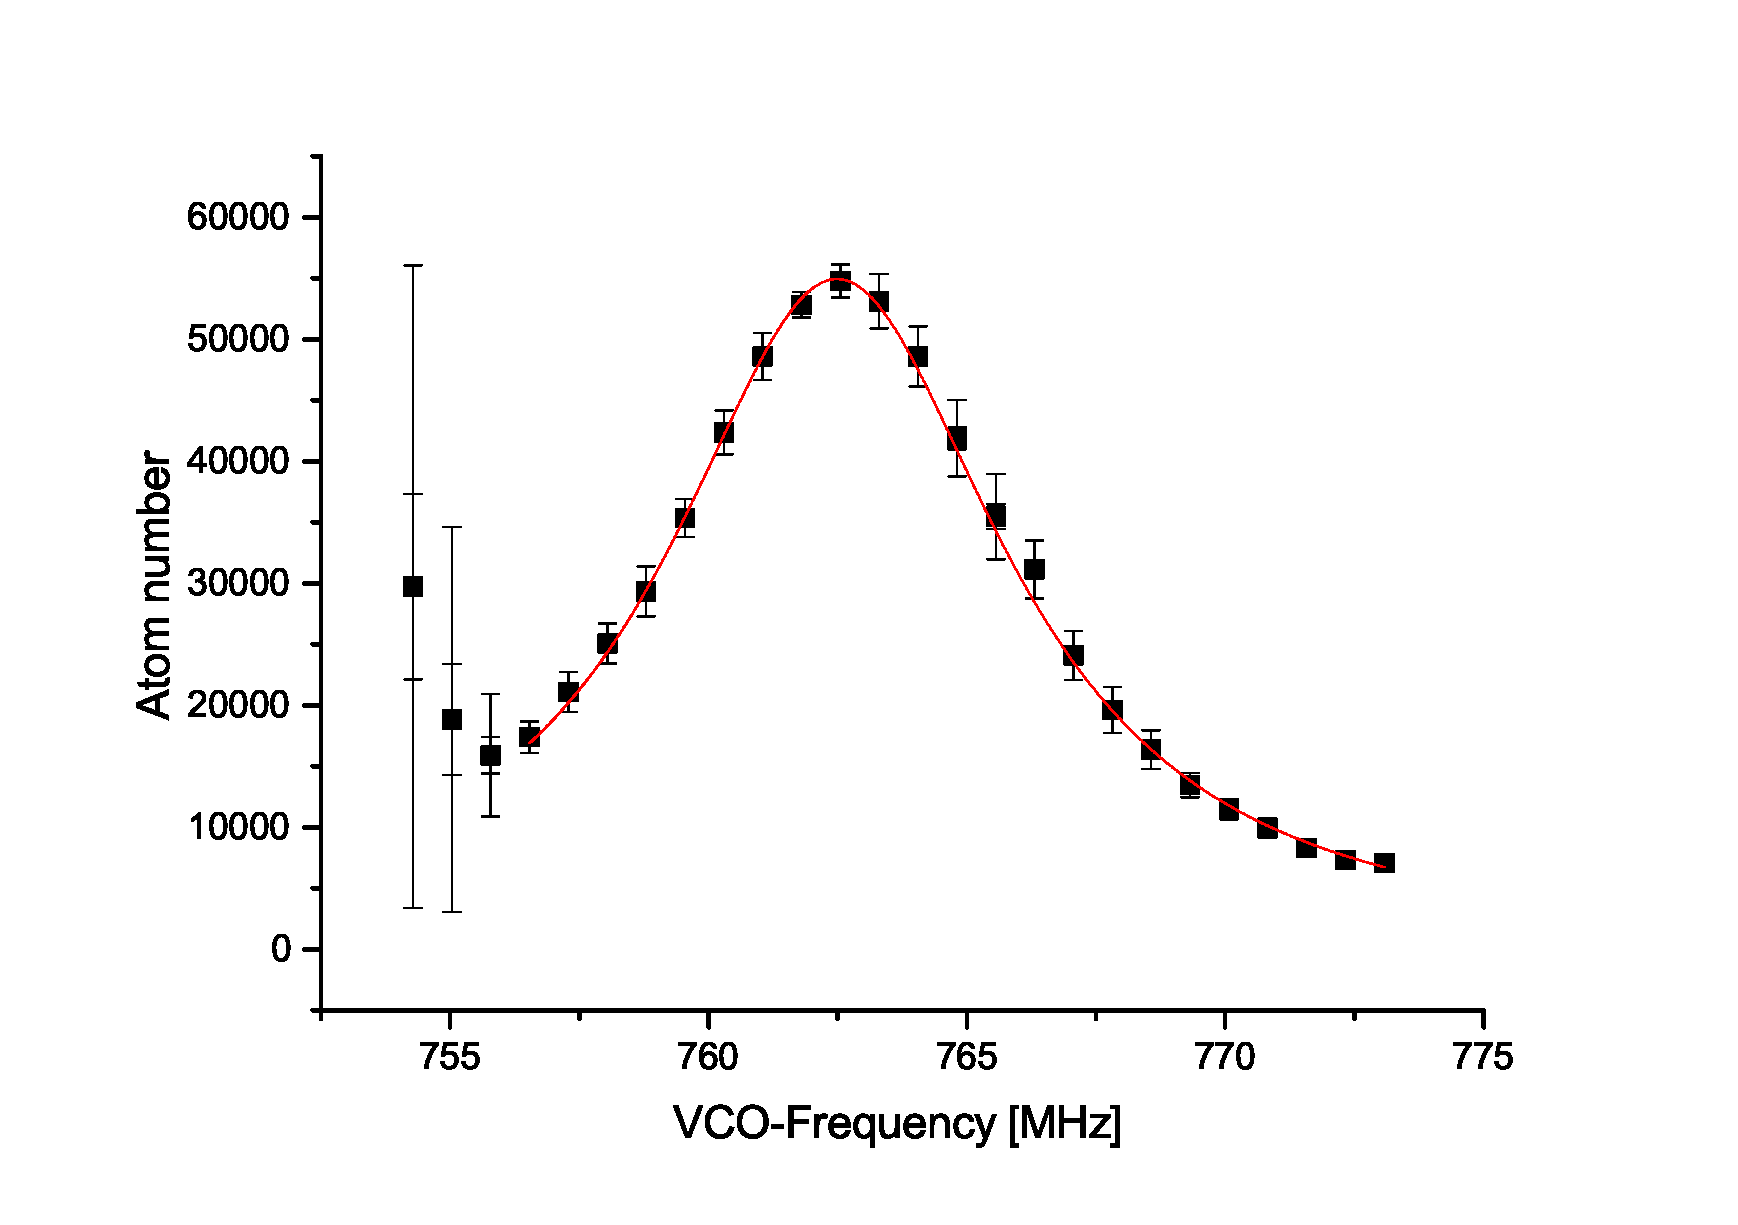
\includegraphics[width=\textwidth]{withodt}
                \caption{Dipole-trap turned on.}
\end{subfigure}


\caption{Resonance peak for the transition: $2s\rightarrow2p_{3/2}, |m_j|=3/2$ at 1070 nm.}
\label{resonance}
\end{figure}

The meassurement of the \textsc{ac}-Stark shift is done in the crossed dipole-trap. To find the resonance peak in the respective setting the atom number is meassured using absorbtion imaging. The frequency of the imaging-laser is hereby scanned over the considered resonance, taking an image for every step in detuning. To find the differential light shift, the pictures are taken either with the activated dipole-trap or with the laser-beams turned off, leaving minimum time of flight in order to get comprehensible results. An example for a resulting image can be seen in figure \ref{resonance}. The resonance shift is clearly visible. The scale has arbitrary fixes and therefore only shows the relative shift. To compare the behaviour as well as the exact values with the theory, different powers were meassured. Note, that the scales show the initial laser-powers. The power in the middle of the trap itself is twice as strong.

\begin{figure}[H]
\centering
\begin{subfigure}[b]{0.8\textwidth}
                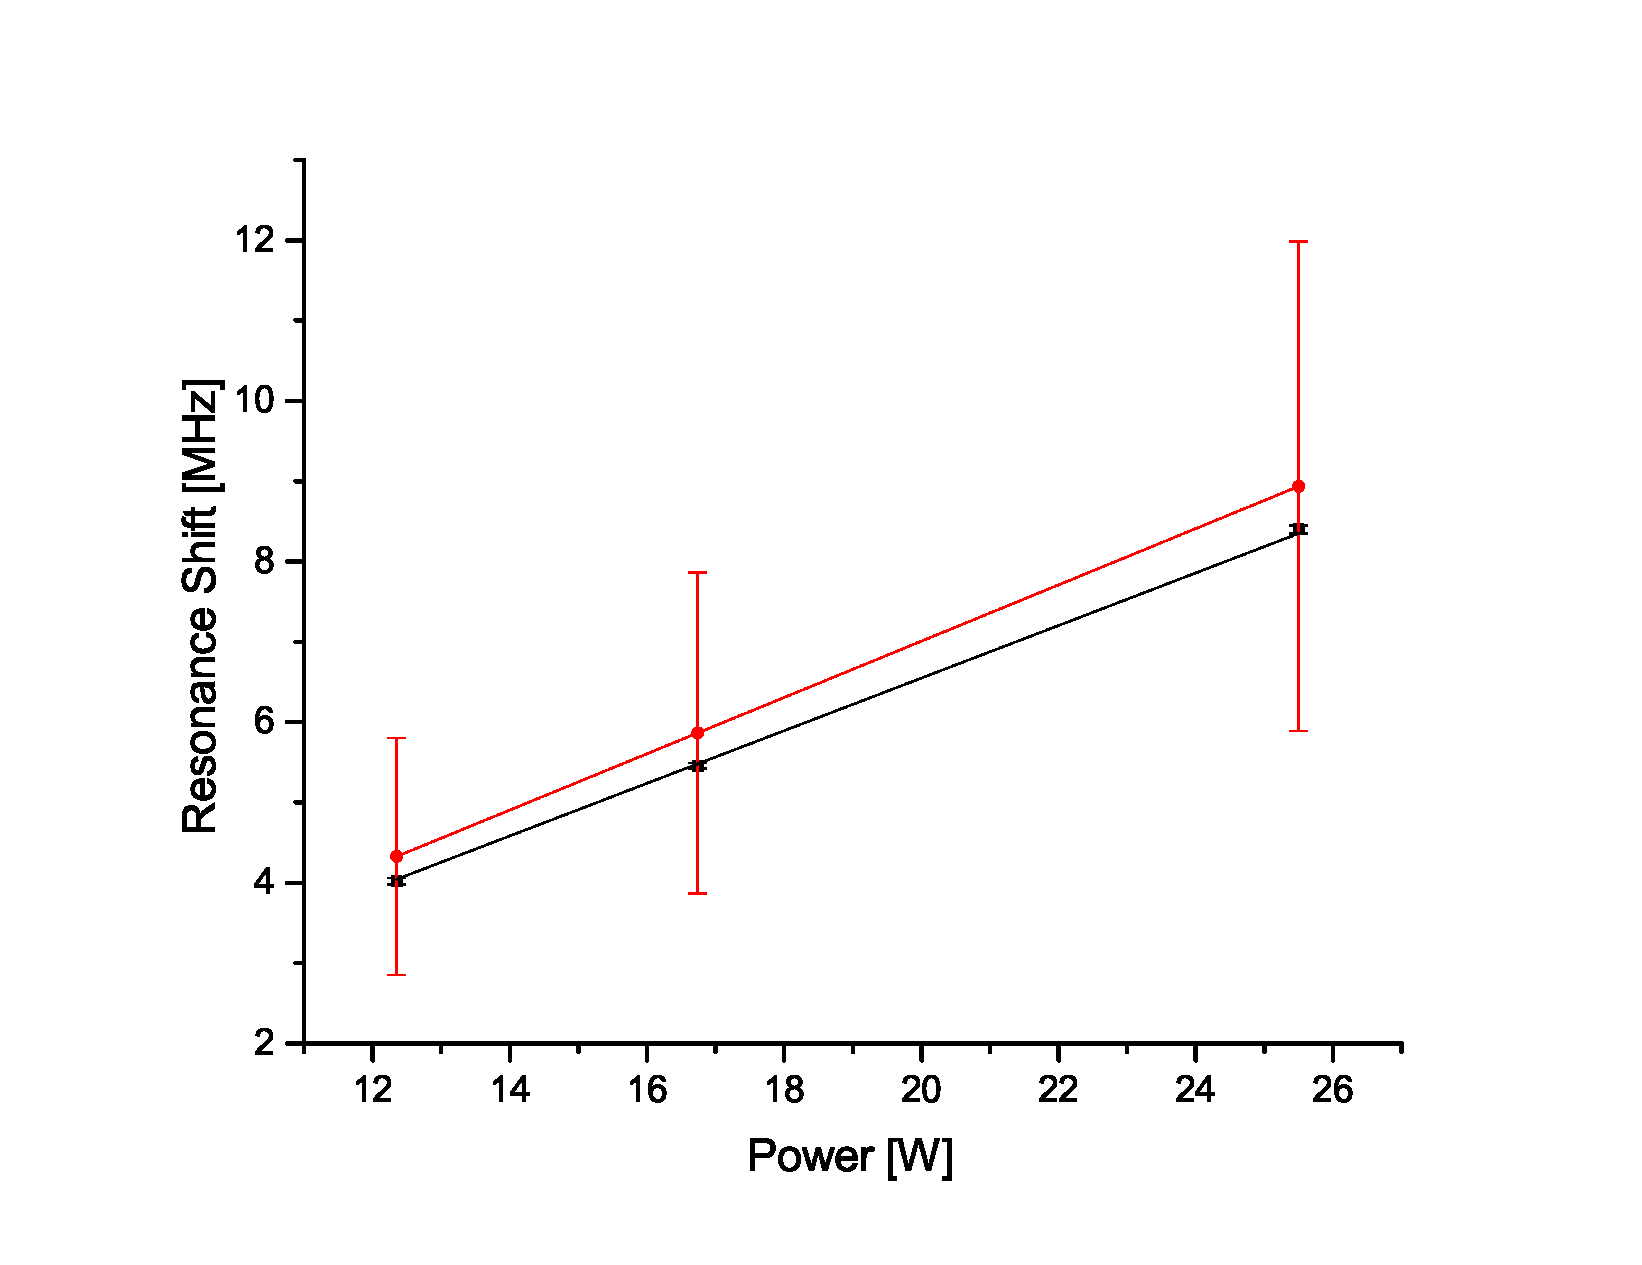
\includegraphics[width=\textwidth]{Shift2}
\end{subfigure}
\caption{Comparison of the differential light-shift in theory (red) and experiment (black) for the D2-line.}
\label{shifts}
\end{figure}

As can be seen in figure \ref{shifts} the shifts are well aligned linearly. The fit was fixed at ($P=0, \Delta E_\mathrm{dif}=0$) and still shows a very good result. The slope is $0.3274\pm 0.0013\unit{MHz/W}$ of initial beam-power, with $\chi^2=1.0$ for the fit. For a more general statement the value is also given in terms of the intensity:
\begin{equation}
\Delta E_\mathrm{dif}/I=0.3717\pm 0.0015\unit{MHz\frac{1}{mW/\mu m^2}}
\end{equation}
Using this value, we also can calculate the trap depth, when knowing the relation of both polarizabilities für gound and excited states.
\begin{align}
U_{\mathrm{g}}=&-\frac{1}{1-\alpha_{\mathrm{e}}/\alpha_{\mathrm{g}}}\cdot \Delta E_\delta\\
U_{\mathrm{e}}=&-\frac{1}{1-\alpha_{\mathrm{g}}/\alpha_{\mathrm{e}}}\cdot \Delta E_\delta
\end{align}
The results of the experiment translate into depths of the trap potential for the $2s$-ground state and $2p_{3/2} m_J=3/2$-excited state with the following values:
\begin{align}
U_g/I=&-(120.32\pm 0.48)\unit{\mu K\ k_B\frac{1}{mW/\mu m^2}}\\
U_e/I=&-(78.05\pm 0.31)\unit{\mu K\ k_B\frac{1}{mW/\mu m^2}}
\end{align}
Also the meassurement can make it possible to find values for other quantities of the trap. The waist of the trap beam for example is usually not exactly easy to meassure, in contrast to its power, that we know with good precision.
\begin{align}
I=&\frac{\epsilon_0 c}{\alpha}\cdot \Delta E_\delta\\\notag\\
w_0=&\sqrt{\frac{2P}{\pi I}}
\end{align}
In this calculation $I$ is the actual maximum-intensity forming the potential and $P$ the initial laser-power in the trap. For the crossed dipole-trap this results in the following waist.
\begin{equation}
w_0=41.383\pm 0.082\unit{\mu m}
\end{equation}

